\documentclass{article}
\usepackage[english]{babel}
\usepackage[T1]{fontenc}
\usepackage{wrapfig}
\usepackage{lscape}
\usepackage{rotating}
\usepackage{graphicx}
\usepackage{listings}
\usepackage{amsmath}
\usepackage{amsfonts}
\usepackage{hyperref}
\usepackage{array}
\usepackage{booktabs}

\title{Chips Operational Semantics}
\author{Anna <3}
\date{\today}

% Source - https://tex.stackexchange.com/a/136050
% Posted by petermeissner, modified by community. See post 'Timeline' for change history
% Retrieved 2026-05-06, License - CC BY-SA 3.0

\newenvironment{myitemize}
{ \begin{itemize}
    \setlength{\itemsep}{0pt}
    \setlength{\parskip}{0pt}
    \setlength{\parsep}{0pt}     }
{ \end{itemize}                  } 


\begin{document}

\maketitle

\section*{Introduction}
This document describes a formal interpretation for each one of the instructions that the Chips language implements. Thank to this description, it becomes possible to draw proofs or formal property definitions for any given Chips model.
In Section~\ref{overview}, we will explore briefly the main programming concepts of the language. Then, Section~\ref{osemantic} precises formally such concepts.

\section{Overview of the language semantics}\label{overview}
Chips describes models of systems executing programs. Therefore, it does not only allows to design algorithms, but it also cares about notions such as ``program embedding'', ``dataflows'' or ``device interconnections''. The simultaneous need to describe both algorithms and devices implies a syntax that mixes elements of both imperative and declarative (synchronous) paradigms. Additionally, the coordination of many components in a single system requires a new kind of (collective) primitives that allow the specification of the data evolution when spread or collected among crowds of devices, where local information matters.


This section is divided in three parts, in relation with the three aspects mentionned above: part~\ref{components} for the definition of the nature and behavior of components of the systems, part~\ref{collective} for the specification of the collective primitive for a smart coordination of distributed processes, and finally, part~\ref{system} for the declaration of the arrangement of components within a complex system.

\subsection{Component description}
The description of components requires two kinds of definitions.
\begin{itemize}
    \item Firstly, a component can be described in terms of what it \emph{does}. To achieve such description, the programmer is provided with the possibility to define \textbf{functions}.
    \item Secondly, a component can be described in terms of what it \emph{is}. To achieve such description, the programmer is provided with the possibility to define \textbf{nodes}.
\end{itemize}
Following subsections (try to) describe briefly the key aspects of Chips functions and nodes.

\subsubsection{Chips Functions}
\label{functions}
Chips function definitions respect the following pattern. They are made of:
\begin{itemize}
    \item a name,
    \item a set of named input parameters,
    \item a list of initializing instructions,
    \item a list of updating instructions,
    \item a set of named output parameters.
\end{itemize}
Input parameters are considered as predefined variables in the context of the updating instruction list of the function or for the defintion of the output expressions. They may have a default value defined in a python-like syntax. Initializing and updating instructions are among:
\begin{itemize}
    \item the declaration instruction (without or with initializing value)
\begin{verbatim}
    <typename> <variable_name>;
    <typename> <variable_name> = <expression>;\end{verbatim}
    \item the assignment instruction
\begin{verbatim}
    <variable_name> = <expression>;\end{verbatim}
    \item the if-then instruction
\begin{verbatim}
    if (<bool_expression>) {
        <list_of_instructions>
    }\end{verbatim}
    \item the if-then-else instruction
\begin{verbatim}
    if (<bool_expression>) {
        <list_of_instructions>
    } else {
        <list_of_instructions>
    }\end{verbatim}
    \item the loop instruction
\begin{verbatim}
    for <variable_decl> in <iterable_expression> {
        <list_of_instructions>
    }\end{verbatim}
\end{itemize}

In Chips, all expressions are considered as arrays. When no dimension is specified for a variable when declared, it is an array of size 1 element.
To build expressions, Chips provides the regular unary and binary operations over integers (\emph{int}), floating point values (\emph{float}) and booleans (\emph{bool}) being described in Figure~\ref{operators}. As Chips is strongly typed, writing expression mixing integers and floating point values without any cast is forbidden. A key aspect related to this strongly typed operation system is that we do not define different operators to distinguish the \emph{euclidian division} and the \emph{floating point division}. The former is associated to the division between integers and the last to floating point values.
All these operators are defined to be applied on arrays of size 1. Using such operators on arrays of different size is undefined.

\begin{figure}
    \centering
    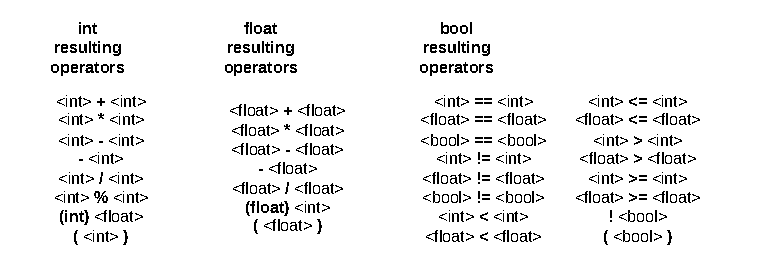
\includegraphics[width=\columnwidth]{imgs/OperatorsList.pdf}
    \caption{Operators implemented in Chips}\label{operators}
\end{figure}

To access the n-th value of an array, one can use the \verb'[<int_index>]' operator. Indices of arrays start at zero:
\begin{verbatim}
float[3] my_var;
my_var[0] = 1.;
my_var[1] = 2.;
my_var[2] = 3.;
float other_var = my_var[1];
\end{verbatim}

Reading the value of a variable that has been declared but hasn't been assigned a value yet is forbidden. To quickly initialize an array of integer, Chips natively provides the functions:
\begin{itemize}
    \item \texttt{zeros($size_{1}, size_{2},$ \ldots)} to return an array only containing $\Pi_{i = 1}^{n} size_{i}$ $0$s,
    \item \texttt{ones($size_{1}, size_{2},$ \ldots)} to return an array only containing $\Pi_{i = 1}^{n} size_{i}$ $1$s,
    \item \texttt{range($size$)} to return an array containing all integers between $0$ and $size-1$ in order.
\end{itemize}

Of course, parameters of these functions have to be positive integers. Otherwise, an error will be raised.
Variable declared in the scope of the initializing instructions of a Chips function are also available in the scope of the updating instruction list and output expressions of that same function.
Figure~\ref{logicalexample} function definition features the usage of different variables in the scope where they are available.
\begin{figure}
    \centering
    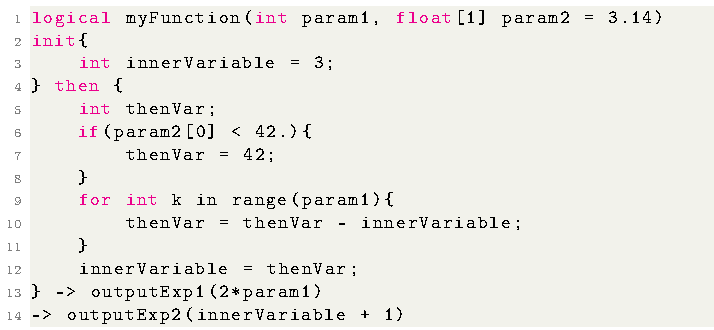
\includegraphics{imgs/functionexample}
    \caption{Definition of a Chips function}\label{logicalexample}
\end{figure}
The keyword logical refers to Chips functions that are not embedded yet. The embedding \emph{link} operation is further defined when it comes to the definition of a Chips model (Section~\ref{modeldef}).

\subsubsection{Chips Nodes}
\label{nodes}
When the need comes to define the features of a component instead of its behavior, we define nodes.
They are made of:
\begin{itemize}
    \item a name,
    \item a list of initializing instructions.
\end{itemize}

In such component definitions, the set of instructions that one can use is containing all the instructions already available for the different code sections of Chips function definitions plus a certain number of instructions that are specific to nodes. Such instructions are:
\begin{itemize}
    \item the contextual declaration instruction (without or with initializing value)
\begin{verbatim}
    ctx <typename> <variable_name>;
    ctx <typename> <variable_name> = <expression>;\end{verbatim}
    \item the channel declaration instruction
\begin{verbatim}
    <channel_type_identifier> <channel_name_identifier>;\end{verbatim}
\end{itemize}

Functions that are embedded in nodes can refer to contextual variables as if they were defined in their scope if their is no name collision between different contextual variables. To do so, we use the \verb'ctx.<ctx_variable_name>' notation in the code sections of the components using it.

Channels are the Chips way to specify the way different nodes are connectable together. They feature a \emph{channel type} being an arbitrarily named type (excluding Chips keywords). During the evaluation of the system description section, these channel types allow to ensure the components connected together are compatible.

The definition of a node is orthogonal to the definition of a function, therefore, Chips provides the mean to define functions that are inherently attached to a node. Such concept is particularly relevant when designing components that emulate the physical behavior of a device. This is why such components are defined with the keyword \emph{physical}. When the programmer needs to design a node as an abstraction for regrouping functions under a single component with shared contextual values, the component has to be defined using the \emph{object} keyword and must be instanciated and linked to by other functions in the system section of a Chips model (we still refer to Section~\ref{modeldef} for further explanations on the concept of linking).

Figure~\ref{objectandphysical} presents an example of definition for a Chips physical function and for a Chips object to illustrate their differences. As a physical function is also a function, it is also featuring inputs, outputs, initializing and updating code sections, just as defined for functions in Section~\ref{functions}.

\begin{figure}
    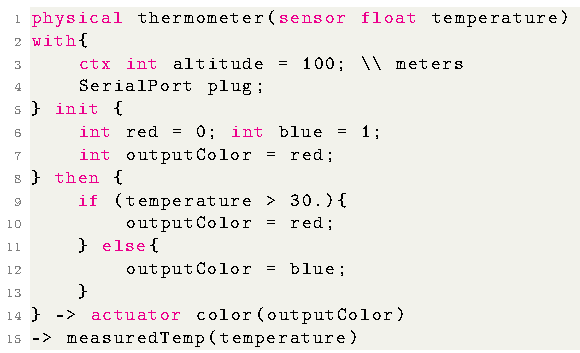
\includegraphics[width=0.6\columnwidth]{imgs/thermometer.pdf}
    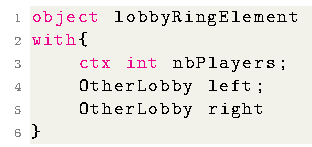
\includegraphics[width=0.35\columnwidth]{imgs/lobbyring.pdf}
    \caption{Two kinds of node definitions, one representing a thermometer component for a cyber-physical system and a second representing an instance of a lobby for a multiplayer server model.}\label{objectandphysical}
\end{figure}

\subsection{Collective functions: \emph{spread} and \emph{collect}}
When propagating data among a network of components, Chips provides the means to define collective functions. They are comparable to the idea of \emph{Streams} in the java language, except that instead of processing the evolution of an accumulated value across logical time, they process the evolution of an accumulated value across logical space (i.e. the stream evolves when it reaches a new components). Such operation is sensitive to the architecture of the model formed, so it cares about the path data takes to go from one node to another. Since the interconnection between nodes is specified by plugging nodes \emph{channels} together, collective functions also make use of the channels defined to specify data propagation.

A collective function definition is composed of:
\begin{itemize}
    \item a direction keyword (\emph{spread} or \emph{collect}),
    \item a name,
    \item a default accumulator definition,
    \item a support node reference,
    \item a stream update code section,
    \item a \emph{target} output expression,
    \item a specification of updated accumulator for each channel of the referenced node.
\end{itemize}

The direction \emph{spread} signify that information transmitted originates from a single component and gets propagated to many others. The direction \emph{collect} signify the information originates from many components and get merged together to become the input of a single one.
The default accumulator definition respects the same rules of the regular Chips function input parameters definition, except that each variable declared as a parameter \textbf{must} be provided with a default value.

To reference a support node, simply use the name of the node definition to use as support.

The target output expression must be of the type of the input of the Chips function that will receive the propagated data. It is annoted with the \texttt{@} symbol.

Updated accumulators must be specified for each channel that is defined for the type of node that the collective function references.
\begin{itemize}
    \item For \emph{spread} operations, all of the channel accumulators but the one that provided the input accumulator to the collective function will be used.
    \item For \emph{collect} operations, only the channel accumulator that goes in the direction of the collecting component will be used.
\end{itemize}

Chips provides a \emph{default} accumulator keyword to define the updated accumulator expression for all the channels that do not have a specification yet.
In the context of collective functions, the set of instructions for the stream update code section is the same as the one from regular functions. However, the semantics of expressions in this context differs in two different ways:
\begin{itemize}
    \item each datatype is enhanced with a new value (represented by the keyword \emph{stop})
    \item some new variables are available by default (the \emph{input} and channel related and variables).
\end{itemize}

\subsubsection{Semantics for \emph{stop}}
The \emph{stop} value is to signify that a variable must not be processed anymore during the propagation. Any component receiving a \emph{stop} signal during a spread operation will propagate the stop signal to warn other connected components that they must keep processing information without waiting for a ``fresh'' value. Any component receiving a \emph{stop} signal during a collect operation will assume the collect operation must be completed using the defaut accumulator instead of a pre-computed one.
The \emph{stop} keyword can be used, during the implementation of the code section of the collective function, as a value of any primitive type. Any operation applied to a \emph{stop} operand will result in the \emph{stop} value.

The stop keyword can be used in any expression of the stream update code section and the updated accumulators expressions.

\subsubsection{Defaultly available variables}
\paragraph{input} is the read-only variable representing the value provided by the Chips function that is the source of the data spread/collected. In the context of a \emph{spread} collective function, it should appear in expressions of the default accumulator definition only. In the context of a \emph{collect} collective function, it should appear in expressions of the stream update code section and/or the updated accumulators expressions. A collective function \textbf{must} feature at least one occurence of the \emph{input} variable.

\paragraph{channel related variables} are a way to refer to accumulators when they are provided through a specific channel of the node. These variables are read-only and can be accessed with the notation
\begin{center}
    \verb'<channel_name>.<accumulator_parameter_name>'
\end{center}
within any expression of the correct type. In case the data read hasn't been initialized because no component is connected through the given channel or because the data transmitted contained a \emph{stop} value, the values of the parameters for that channel are the default values defined for the accumulator of this collective function definition.

Figure~\ref{collectexample} presents an example of definition for a collective function featuring all the metionned characteristics above. This example is pretty absurdly complicated for the sake of demonstrating all the usable features of collective function definitions. For this example to be fully functional, we assume that contextual values are previously set by other Chips functions linked to each instance of \emph{ContainerObject}. We also assume the objects are correctly connected together by associating each channel of a given \emph{ContainerObject} to at most one channel of another \emph{ContainerObject}.

It is worth noting that for each channeled accumulator defined, the types of the provided expression respect the types of the default accumulator. If it hasn't been the case, an error would have been raised.
\begin{figure}
    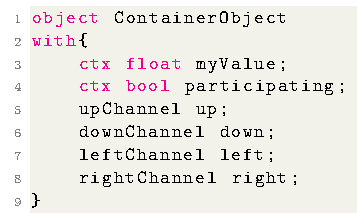
\includegraphics[width=0.3\columnwidth]{imgs/ContainerObject.pdf}
    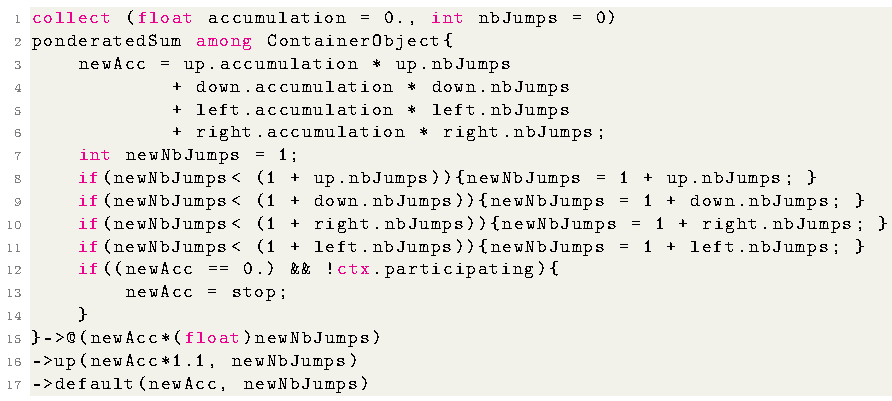
\includegraphics[width=0.7\columnwidth]{imgs/collectivefunctionexample.pdf}
    \caption{An object definition and a collective function to compute a sum of all the functions among the defined object, ponderated by the longest path to a leaf of the tree formed by the configuration used to collect data, putting an emphasis on data propagated via the \emph{up} channel.}\label{collectexample}
\end{figure}

\subsection{Definition of a Chips model}\label{modeldef}
// TO BE CONTINUED

\section{Operational Semantic}\label{osemantic}

This section is dedicated to mathematically describe the elements of the Chips language that were described earlier in a less formal way.
After having introduced the formalism that is used in this document, we will define the Chips partially synchronous semantics into two sections. Section~\ref{components} describes the imperative semantics of Chips, which is mostly relevant during the description of the components and the collective functions. Section~\ref{system} describes the synchronous semantics of Chips, which is to be applied during the description of the Chips models evaluation, \emph{i.e.} in the \texttt{system} section evaluation of a Chips file.

\subsection{Formalism and Notations}

The Chips language uses three kinds of primitive types being \emph{integers}, \emph{floating point values} and \emph{booleans}. The sets of all possible values of these types will respectively be denoted \emph{int}, \emph{float} and \emph{bool}, as in current general purpose programming languages. We assume their encoding being implementation dependant so we will not further describe these sets or specific restrictions applied to the operations applied to them.

Let $N$ (as in name) be the set of all possible string sequences that are valid names. From the Chips grammar (Appendix~\ref{grammar}), we see that this set is exactly the language generated from the regular expression \texttt{[a-zA-Z][a-zA-Z\_]*}, deprived of the set of the Chips keywords.

To make the difference between both paradigms applied in the context of Chips, we must define two separated type environments. We will call them:
\begin{itemize}
    \item $\Gamma_{imp}$ for the imperative code sections related to the definition of Chips functions and nodes, and 
    \item $\Gamma_{sync}$ for the synchronous code section that is the system section.
\end{itemize}

\noindent Let $Val$ be the set of all possible values of variables:
\[
Val = \bigcup_{i=1}^{n} int^{i} \cup float^{i} \cup bool^{i}
\]
With $n \in \mathbb{N}$ being an arbitrarily big number, processor architecture dependant.\\
We can then define the \emph{stop} value as a distinguished element such that $stop \not\in Val$ and $V_c$, the set of all possible values in the context of collective functions stream update code section as:
\[
Val_c = Val \cup stop
\]
$N$ and $Val_c$ now allow us to define the set $Var$ of all the functions that map names of potential variables to their value:
\[
Var: N \mapsto Val_c
\]
From this set, we will define the possible memory states of a process $M$ as the powerset of $Var$:
\[
M = \mathcal{P}(Var)
\]
Now, we can focus on the definition of the programs that are meant to be executed by the processes. To do so, let us introduce the set of well formed sequences of Chips instructions as $I$. In our context, ``well formed'' signifies that it doesn't raise a syntax error, wrong model composition error or an error due to the unavailibility of:
\begin{itemize}
    \item a variable in the memory,
    \item an operator of the matching type and operand types in the language,
    \item a function call refering to one of the predefined Chips functions,
    \item a logical/physical/object block of the matching name in the context,
    \item a logical/physical/object block instance of the matching name in the context.
\end{itemize}

All the definitions above allow us to draw a general pattern for the formalisation of evaluation rules of imperative code being:
\[
\Gamma \vdash \langle m_i, \pi \rangle \rightarrow \langle m_{i+1}, \pi' \rangle
\]
Having:
\begin{myitemize}
    \item[] $i < n \in \mathbb{N}$,
    \item[] $m_i, m_{i+1} \in M$,
    \item[] $\pi, \pi' \in I$,
    \item[] and $\Gamma$ as the type environment of the evaluated instructions
\end{myitemize}

Such formula reads ``In the environment of $\Gamma$, the memory state $m_i$ and the set of instructions $\pi$ can be interpreted as the memory state $m_{i+1}$ and the set of instructions $\pi'$''.

The semantics of the following Chips expressions and instructions are similar to many other standard programming languages:
\begin{verbatim}
+ (plus), - (minus and unary minus), * (multiply), / (euclidian 
and real division), % (modulo), ! (not), && (and), || (or), == 
(equals), != (different), <= (lower or equal), >= (greater or 
equal), < (greater than), > (lower than), variable 
declaration/assignment/reading, (predefined) function call,
[](array access), if and if-else structures\end{verbatim}
They will not be covered by this document and we refer to~\cite{plotkin1981structural} for a detailed explanation of their evaluation.

% \[
% \cfrac{}{\langle m_i, \pi \rangle \rightarrow \langle m_{i+1}, \pi' \rangle}
% \]

\subsection{Operational semantics of Chips imperative code}\label{componentsos}

\subsubsection{Expressions}

\paragraph{\emph{int/float} casting}
\paragraph{Contextual variable reading/assignment}
\paragraph{Predefined function call}

\subsubsection{Instructions}

\paragraph{\emph{for} loop instruction}

\subsubsection{On the absence of \emph{while} loops}

\subsection{Operational semantics of Chips system description}\label{systemos}

\subsubsection{System architecture instructions}

\paragraph{Link instruction}

\paragraph{Channel assignment}

\subsubsection{Synchronous L/R values}

\paragraph{Functional block logical/physical input}

\paragraph{Functional block logical/physical output}

\paragraph{Collective primitives}

\paragraph{Constant expressions}


\newpage
\appendix
\section{Chips grammar}\label{grammar}
The current syntax of the language is defined hereafter in the style of ANTLR4 (BNF enhanced with regular expression elements).
\begin{verbatim}
grammar Chips;
program
    : preamble* system? EOF
    ;
system
    : SYSTEM_KW L_CURL
        s_statement*
      R_CURL
    ;
preamble
    : object_def
    | function_def
    | collective_op_def
    ;
object_def
    : OBJECT_KW IDENTIFIER with_section
    ;
node_mapping
    : HAVING_KW IDENTIFIER AS_KW IDENTIFIER SEMICOL
    ;
function_def
    : l_function_def
    | p_function_def
    ;
collective_op_def
    : c_signature L_CURL
        c_statement*
      R_CURL
      ARROW TARGET_KW L_PARENTH c_expr (COMMA c_expr)* R_PARENTH
      c_output+
    ;
c_output
    : ARROW DEFAULT_KW L_PARENTH c_expr (COMMA c_expr)* R_PARENTH
    | ARROW IDENTIFIER L_PARENTH c_expr (COMMA c_expr)* R_PARENTH
    ;
l_function_def
    : LOGICAL_KW IDENTIFIER L_PARENTH 
        (df_parameter_decl (COMMA df_parameter_decl)*)? R_PARENTH
        init_section
        then_section
        named_output*
    ;
p_function_def
    : PHYSICAL_KW IDENTIFIER L_PARENTH 
        (pdf_parameter_decl (COMMA pdf_parameter_decl)*)? R_PARENTH
        with_section
        init_section
        then_section
        p_named_output*
    ;
c_signature
    : c_keywords L_PARENTH 
        (cdf_defaulted_decl (COMMA cdf_defaulted_decl)*)? R_PARENTH
        IDENTIFIER AMONG_KW IDENTIFIER
    ;
c_keywords
    : SPREAD_KW
    | COLLECT_KW
    ;
with_section
    : WITH_KW L_CURL
        with_statement*
      R_CURL
    ;
with_statement
    : IDENTIFIER IDENTIFIER SEMICOL
    | CTX_KW df_type suffixes IDENTIFIER (ASSIGN expr)? SEMICOL
    | statement
    ;
init_section
    : INIT_KW L_CURL
        (statement)*
      R_CURL
    ;
then_section
    : THEN_KW L_CURL
        (statement)*
      R_CURL
    ;
expr
    : expr0 LT expr
    | expr0 GT expr
    | expr0 LEQ expr
    | expr0 GEQ expr
    | expr0 NEQ expr
    | expr0 EQ  expr
    | expr0 AND expr
    | expr0 OR expr
    | expr0
    ;
expr0
    : expr01 PLUS expr0
    | expr01 MINUS expr0
    | expr01
    ;
expr01
    : MINUS expr1
    | expr1
    ;
expr1
    : expr2 TIMES expr1
    | expr2 DIV expr1
    | expr2 MOD expr1
    | NOT expr2
    | expr2
    ;
expr2
    : INT
    | FLOAT
    | BOOL
    | IDENTIFIER suffixes
    | L_PARENTH expr R_PARENTH
    | CTX_KW PERIOD IDENTIFIER suffixes
    | IDENTIFIER L_PARENTH (expr (COMMA expr)*)? R_PARENTH
    | cast
    ;
cast
    : L_PARENTH df_type R_PARENTH expr
    ;
c_expr
    : c_stopless_expr
    | STOP_KW
    ;
c_stopless_expr
    : c_stopless_expr0 LT c_stopless_expr
    | c_stopless_expr0 GT c_stopless_expr
    | c_stopless_expr0 LEQ c_stopless_expr
    | c_stopless_expr0 GEQ c_stopless_expr
    | c_stopless_expr0 NEQ c_stopless_expr
    | c_stopless_expr0 EQ c_stopless_expr
    | c_stopless_expr0 AND c_stopless_expr
    | c_stopless_expr0 OR c_stopless_expr
    | c_stopless_expr0
    ;
c_stopless_expr0
    : c_stopless_expr01 PLUS c_stopless_expr0
    | c_stopless_expr01 MINUS c_stopless_expr0
    | c_stopless_expr01
    ;
c_stopless_expr01
    : MINUS c_stopless_expr1
    | c_stopless_expr1
    ;
c_stopless_expr1
    : c_stopless_expr2 TIMES c_stopless_expr1
    | c_stopless_expr2 DIV c_stopless_expr1
    | c_stopless_expr2 MOD c_stopless_expr1
    | NOT c_stopless_expr2
    | c_stopless_expr2
    ;
c_stopless_expr2
    : IDENTIFIER c_suffixes
    | INT
    | FLOAT
    | BOOL
    | INPUT_KW
    | CTX_KW PERIOD IDENTIFIER c_suffixes
    | IDENTIFIER PERIOD IDENTIFIER c_suffixes
    | IDENTIFIER L_PARENTH (c_expr (COMMA c_expr)*)? R_PARENTH
    | L_PARENTH c_stopless_expr R_PARENTH
    | c_cast
    ;
c_cast
    : L_PARENTH df_type R_PARENTH c_stopless_expr
    ;
suffixes
    : (L_SQUA expr R_SQUA)*
    ;
c_suffixes
    : (L_SQUA c_stopless_expr R_SQUA)*
    ;
s_suffixable_expr
    : IDENTIFIER
    | IDENTIFIER (L_PARENTH (expr (COMMA expr)*)? R_PARENTH)?
    | block PERIOD IDENTIFIER
    ;
block
    : IDENTIFIER suffixes
    ;
loop_in
    :  IDENTIFIER (L_PARENTH (expr (COMMA expr)*)? R_PARENTH)?
    ;
loop_statement
    : FOREACH_KW IDENTIFIER IN_KW loop_in L_CURL
        statement*
      R_CURL
    ;
c_loop_statement
    : FOREACH_KW IDENTIFIER IN_KW loop_in L_CURL
        c_statement*
      R_CURL
    ;
s_loop_statement
    : FOREACH_KW IDENTIFIER IN_KW s_suffixable_expr L_CURL
        s_statement*
      R_CURL
    ;
if_else_statement
    : if_statement
      ELSE_KW L_CURL
        (statement)*
      R_CURL
    ;
s_if_else_statement
    : s_if_statement
      ELSE_KW L_CURL
        s_statement*
      R_CURL
    ;
c_if_else_statement
    : c_if_statement
      ELSE_KW L_CURL
        c_statement*
      R_CURL
    ;
if_statement
    : IF_KW L_PARENTH expr R_PARENTH L_CURL
        (statement)*
      R_CURL
    ;
s_if_statement
    : IF_KW L_PARENTH expr R_PARENTH L_CURL
        s_statement*
      R_CURL
    ;
c_if_statement
    : IF_KW L_PARENTH c_expr R_PARENTH L_CURL
        c_statement*
      R_CURL
    ;
statement
    : df_type suffixes IDENTIFIER (ASSIGN expr)? SEMICOL
    | IDENTIFIER suffixes ASSIGN expr SEMICOL
    | CTX_KW PERIOD IDENTIFIER suffixes ASSIGN expr SEMICOL
    | loop_statement
    | if_else_statement
    | if_statement
    ;
s_statement
    : IDENTIFIER suffixes IDENTIFIER SEMICOL
    | block PERIOD IDENTIFIER L_PARENTH s_expr R_PARENTH SEMICOL
    | LINK_KW IDENTIFIER suffixes TO_KW IDENTIFIER suffixes SEMICOL
    | s_loop_statement
    | s_if_else_statement
    | s_if_statement
    | statement
    ;
s_expr
    : block PERIOD IDENTIFIER
    | collective_operation block PERIOD IDENTIFIER
    | expr
    ;
collective_operation
    : L_PARENTH IDENTIFIER R_PARENTH
    ;
c_statement
    : cdf_full_declaration SEMICOL
    | IDENTIFIER c_suffixes ASSIGN c_expr SEMICOL
    | CTX_KW PERIOD IDENTIFIER c_suffixes ASSIGN c_expr SEMICOL
    | c_loop_statement
    | c_if_else_statement
    | c_if_statement
    ;
named_output
    : ARROW IDENTIFIER L_PARENTH expr (COMMA expr)* R_PARENTH
    ;
p_named_output
    : ARROW ACTUATOR_KW IDENTIFIER L_PARENTH expr (COMMA expr)* R_PARENTH
    | named_output
    ;
df_parameter_decl
    : df_type suffixes IDENTIFIER (ASSIGN expr)?
    ;
df_type
    : INT_KW
    | FLOAT_KW
    | BOOL_KW
    ;
pdf_parameter_type
    : df_type suffixes
    | SENSOR_KW df_type suffixes
    ;
pdf_parameter_decl
    : pdf_parameter_type IDENTIFIER (ASSIGN expr)?
    ;
cdf_defaulted_decl
    : df_type suffixes IDENTIFIER ASSIGN c_expr
    ;
cdf_full_declaration
    : df_type suffixes IDENTIFIER (ASSIGN c_expr)?
    ;
SYSTEM_KW           : 'system'|'SYSTEM';
INT_KW              : 'int';
FLOAT_KW            : 'float';
BOOL_KW             : 'bool';
LOGICAL_KW          : 'logical';
PHYSICAL_KW         : 'physical';
AS_KW               : 'as';
INIT_KW             : 'init';
THEN_KW             : 'then';
FOREACH_KW          : 'for';
IN_KW               : 'in';
IF_KW               : 'if';
ELSE_KW             : 'else';
TO_KW               : 'to';
LINK_KW             : 'link';
HAVING_KW           : 'having';
INPUT_KW            : 'input';
STOP_KW             : 'stop';
AMONG_KW            : 'among';
SPREAD_KW           : 'spread';
COLLECT_KW          : 'collect';
CTX_KW              : 'ctx';
OBJECT_KW           : 'object';
WITH_KW             : 'with';
BY_KW               : 'by';
TARGET_KW           : '@';
DEFAULT_KW          : 'default';
USING_KW            : 'using';
ACTUATOR_KW         : 'actuator';
SENSOR_KW           : 'sensor';
ARROW               : '->';
PLUS                : '+';
MINUS               : '-';
TIMES               : '*';
DIV                 : '/';
MOD                 : '%';
LT                  : '<';
GT                  : '>';
EQ                  : '==';
LEQ                 : '<=';
GEQ                 : '>=';
NEQ                 : '!=';
AND                 : '&&';
OR                  : '||';
NOT                 : '!';
ASSIGN              : '=';
COMMA               : ',';
SEMICOL             : ';';
L_PARENTH           : '(';
R_PARENTH           : ')';
L_CURL              : '{';
R_CURL              : '}';
L_SQUA              : '[';
R_SQUA              : ']';
COLUMN              : ':';
PERIOD              : '.';
BOOL                : 'true'| 'false';
fragment DIGIT      : [0-9] ;
fragment DOTTED_NUMBER
    : '.'DIGIT+
    | DIGIT+'.'DIGIT*
    ;
fragment ID_START   : [a-zA-Z];
fragment ID_NEXT    : [a-zA-Z0-9_];
FLOAT               : DOTTED_NUMBER;
INT                 : DIGIT+;
IDENTIFIER          : ID_START ID_NEXT*;
NEWLINE : ('\r'? '\n')+ -> skip ;
WS          : [ \t\r]+ -> skip ;
COMMENT     : '//' ~[\r\n]* -> skip ;
\end{verbatim}
\end{document}